\chapter{深度学习}

\begin{figure}[htp]
    \centering
    \includegraphics[width=14cm]{figure/深度学习模型实现流程.png}
    \caption{\kaishu 深度学习模型实现流程}\label{Fig: 深度学习模型实现流程}
\end{figure}

\section{数据处理}
% \begin{itemize}
%     \item 
%     \item 
%         \begin{equation*}
%         \mbox{划分数据集}
%         \begin{cases}
%             \mbox{train\_set(训练集):用于确定模型参数。}\\
%             \mbox{val\_set(验证集):用于调节模型超参数(如多个网络结构、正则化权重的最优选择)。}\\
%             \mbox{test\_set(测试集):用于估计应用效果(尽量使用未在模型中应用过的数据)。}
%         \end{cases}
%         \end{equation*}
%         其中训练集必包含训练数据(images)部分和标签(labels 或 ground truthz)部分。

%         验证: validate
%         测试: test 或 evaluate
%     \item 
%         \begin{equation*}
%         \mbox{训练样本集乱序\footnote{通过大量实验发现,模型对最后出现的数据印象更加深刻。训练数据导入后,越接近模型训练结束,最后几个批次数据对模型参数的影响越大。为了避免模型记忆影响训练效果,需要进行样本乱序操作。}}
%         \begin{cases}
%             \mbox{建立顺序编号的ID集合index\_list}\\
%             \mbox{将index\_list乱序}\\
%             \mbox{按乱序后的顺序读取数据}
%         \end{cases}
%         \end{equation*}
%         为什么要乱序?

%         % 实现乱序的操作:
%         % random.shuffle(index\_list)
%     \item 
%         \begin{equation*}
%         \mbox{生成批次数据}
%         \begin{cases}
%             \mbox{设置合理的batch\_size}\\
%             \mbox{将数据shape变为(batch\_size, image\_size)的np.array}\\
%             \mbox{使用python的yield生成器返回数据}
%         \end{cases}
%         \end{equation*}
%     \item 校验数据有效性
% \end{itemize}
    
    \begin{equation*}
    \begin{cases}
    \mbox{读入数据}\\
    \mbox{划分数据集}
        \begin{cases}
            \mbox{train\_set(训练集):用于确定模型参数。}\\
            \mbox{val\_set(验证集):用于调节模型超参数(如多个网络结构、正则化权重的最优选择)。}\\
            \mbox{test\_set(测试集):用于估计应用效果(尽量使用未在模型中应用过的数据)。}
        \end{cases}\\
    \mbox{训练样本集乱序}\footnote{通过大量实验发现,模型对最后出现的数据印象更加深刻。训练数据导入后,越接近模型训练结束,最后几个批次数据对模型参数的影响越大。为了避免模型记忆影响训练效果,需要进行样本乱序操作。}
        \begin{cases}
            \mbox{建立顺序编号的ID集合index\_list}\\
            \mbox{将index\_list乱序}\\
            \mbox{按乱序后的顺序读取数据}
        \end{cases}\\
    \mbox{生成批次数据}
        \begin{cases}
            \mbox{设置合理的batch\_size}\\
            \mbox{将数据shape变为(batch\_size, image\_size)的np.array}\\
            \mbox{使用python的yield生成器返回数据}
        \end{cases}\\
    \mbox{校验数据有效性}
        \begin{cases}
            \mbox{机器校验: assert 图片 与 标签 维度相同}\\
            \mbox{人工校验: print 数据看格式是否符合预期}
        \end{cases}
    \end{cases}
    \end{equation*}

    某基于MNIST数据集的数据生成器的代码实现如下。
    % \begin{lstlisting}[language={Python}]
    \begin{python}
# 定义数据生成器,返回批次数据
def load_data(mode='train'):
    datafile = './work/mnist.json.gz'
    print('loading mnist dataset from {} ......'.format(datafile))
    # 加载json数据文件
    data = json.load(gzip.open(datafile))
    print('mnist dataset load done')
   
    # 读取到的数据区分训练集,验证集,测试集
    train_set, val_set, eval_set = data
    if mode=='train':
        # 获得训练数据集
        imgs, labels = train_set[0], train_set[1]
    elif mode=='valid':
        # 获得验证数据集
        imgs, labels = val_set[0], val_set[1]
    elif mode=='eval':
        # 获得测试数据集
        imgs, labels = eval_set[0], eval_set[1]
    else:
        raise Exception("mode can only be one of ['train', 'valid', 'eval']")
    print("训练数据集数量: ", len(imgs))
    
    # 校验数据
    imgs_length = len(imgs)

    assert len(imgs) == len(labels), \
          "length of train_imgs({}) should be the same as train_labels({})".format(len(imgs), len(labels))
    
    # 获得数据集长度
    imgs_length = len(imgs)
    
    # 定义数据集每个数据的序号,根据序号读取数据
    index_list = list(range(imgs_length))
    # 读入数据时用到的批次大小
    BATCHSIZE = 100
    
    # 定义数据生成器
    def data_generator():
        if mode == 'train':
            # 训练模式下打乱数据
            random.shuffle(index_list)
        imgs_list = []
        labels_list = []
        for i in index_list:
            # 将数据处理成希望的类型
            img = np.array(imgs[i]).astype('float32')
            label = np.array(labels[i]).astype('float32')
            imgs_list.append(img) 
            labels_list.append(label)
            if len(imgs_list) == BATCHSIZE:
                # 获得一个batchsize的数据,并返回
                yield np.array(imgs_list), np.array(labels_list)
                # 清空数据读取列表
                imgs_list = []
                labels_list = []
    
        # 如果剩余数据的数目小于BATCHSIZE,
        # 则剩余数据一起构成一个大小为len(imgs_list)的mini-batch
        if len(imgs_list) > 0:
            yield np.array(imgs_list), np.array(labels_list)
    return data_generator
    \end{python}

    % \end{lstlisting}

\section{模型设计}

    \subsection{多层感知机}
    多层感知器(Multi Layer Perceptron,即 MLP)除了一个输入层和一个输出层以外,包括至少一个隐藏层。多层感知器用来模拟一个非线性函数。


    \subsection{卷积神经网络}

    

\section{训练配置}


    \subsection{反向传播}

    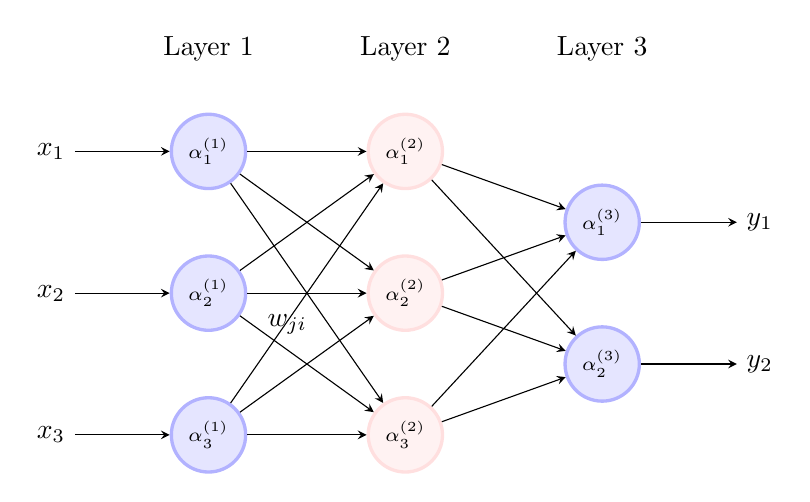
\begin{tikzpicture}
		[L1Node/.style={circle,draw=blue!30,fill=blue!10,very thick, minimum size=10pt},
		L2Node/.style={circle,draw=pink!50,fill=pink!20,very thick, minimum size=10pt}]
		
		% 画输入层结点
		\foreach \x in {1,...,3}  % 循环,使得\x的值依次等于1,2,3
		% \node[结点的样式](结点的名称)at(结点的坐标){结点的内容}
		\node[L1Node] (a_\x) at (0,-1.8*\x){\scriptsize $\alpha^{(1)}_\x$};  
		
		% 画隐藏层结点
		\foreach \x in {1,...,3}
		\node[L2Node] (b_\x) at (1*2.5,-1.8*\x){\scriptsize $\alpha^{(2)}_\x$};
		
		% 画输出层结点
		\foreach \y in {1,2}
		\node[L1Node] (c_\y) at (2*2.5,-1.8*\y-1.8/2){\scriptsize $\alpha^{(3)}_\y$};

        % 添加说明表示
        \node[]at(0*2.5,-0.5){Layer 1};
        \node[]at(1*2.5,-0.5){Layer 2};
        \node[]at(2*2.5,-0.5){Layer 3};

        % 输入特征x
		\foreach \x in {1,2,3}
		\node(x_\x)at(-2,-1.8*\x){$x_\x$};
		
		% 输出数值y
		\node(y_1)at(2*2.5+2,-1.8*1-1.8/2){$y_1$};
		\node(y_2)at(2*2.5+2,-1.8*2-1.8/2){$y_2$};
		
		% 输入特征值与输入层之间的连线
		\foreach \x in {1,2,3} 
		\draw[-stealth](x_\x)--(a_\x);
		
		% 链接输入层到隐藏层之间的连线
		\foreach \x in{1,2,3}
		{\foreach \z in{1,2,3}
			% \draw[线的样式:-{stealth[sep=1pt]}为带箭头的线,[sep箭头距离]
			\draw[-stealth](a_\x)--(b_\z);	
		}
		
		% 链接隐藏层到输出层之间的连线
		\foreach \z in{1,2,3}
		{\foreach \y in{1,2}
			\draw[-stealth](b_\z)--(c_\y);	
		}
		
		% 输出y与输出层之间的连线
		\draw[-stealth](c_1)--(y_1);
		\draw[-stealth](c_2)--(y_2);
		
		% % 添加权值w
		% % \node[结点的样式](结点的名称)at(结点的坐标){结点的内容}
		% \node[](w_1) at (1,-0.65){$w_{41}$};
		% \node[](w_2) at (1,-1.15){$w_{42}$};
		% \node[](w_3) at (1,-1.65){$w_{43}$};
		
		
		% % 隐藏层公式
		% \node[](z) at (2,0.3){$z_j=sigmoid(a_j)$};

		
		% % 输出层公式
		% \node[](y) at (4,-0.5){$y_k=sigmoid(b_k)$};
		

		\node[](w_ji)at(1,-4){$w_{ji}$};
		
	\end{tikzpicture}

    \begin{itemize}
        \item 计算梯度
            \begin{equation}
                \bm{g} \leftarrow \partial_{(\bm{W},b)} \frac{1}{|\mathcal{B}|} \sum_{i\in\mathcal{B}}{L\left(\bm{x}^{(i)},\bm{y}^{(i)},\bm{W},b\right)}
            \end{equation}
        \item 更新参数
            \begin{equation}
                (\bm{W},b) \leftarrow (\bm{W},b) - \eta \bm{g} 
            \end{equation}
    \end{itemize}


    \subsection{特征标准化}

    为了解决输入样本中各个维度的数值差异较大导致 error surface 形状扭曲, 给 gradient descent 带来困难 的问题,引入特征标准化(\emph{Feature Normalization})的方法。

    \begin{itemize}
        \item Batch Normalization
        \item Layer Normalization
        \item lnstance Normalization
        \item Group Normalization
        \item Weight Normalization
        \item Spectrum Normalization
    \end{itemize}

    其中一个常用的标准化方法为 Batch Normalization (BN) 。BN 一次对一个 Batch (记作$\mathcal{B}$,其中第$i$个样本为$N_e\times 1$列向量$\bm{x}^{(i)},\,i=1,\cdots,N_B$) 的输入样本的每一个维度作\emph{standard deviation normalization}:
    \begin{equation}
        % \tilde{\bm{x}}^{(i)}=\frac{\bm{x}^{(i)}-\bm{\mu}}{\bm{\sigma}}
        \tilde{\bm{x}}^{(i)}=\frac{\bm{x}^{(i)}-\mathrm{E}\left[\bm{x}^{(:)}\right]}{\sqrt{\mathrm{Var}\left[\bm{x}^{(:)}\right]}}
    \end{equation}
    % 其中,$\bm{\mu},\bm{\sigma}$分别为一个 Batch 的样本 按对应维度求出的均值和标准差 所组成的向量,其 shape 与 每一个样本的 shape 相同。
    % \begin{subequations}    
    % \begin{equation}
    %     \bm{\mu}=\frac{1}{N_B}\sum_{i=1}^{N_B}{\bm{x}^{(i)}}
    % \end{equation}
    % \begin{equation}
    %     \bm{\sigma}=
    % \end{equation}
    % \end{subequations}
    其中,$\mathrm{E}\left[\bm{x}^{(:)}\right]$ 表示对一个 Batch 内全部样本在同一个维度上求均值,得到一个$N_e\times 1$列向量。求方差$\mathrm{Var}\left[\bm{x}\right]$的过程同理。
        
\section{模型保存}


\section{模型预测}